% SPDX-FileCopyrightText: 2026 Cyprien PIERRE
% SPDX-License-Identifier: CC-BY-4.0
\documentclass[tikz,border=5pt]{standalone}
\usepackage[T1]{fontenc}
\usepackage{lmodern}
\usetikzlibrary{arrows.meta,positioning}
\begin{document}
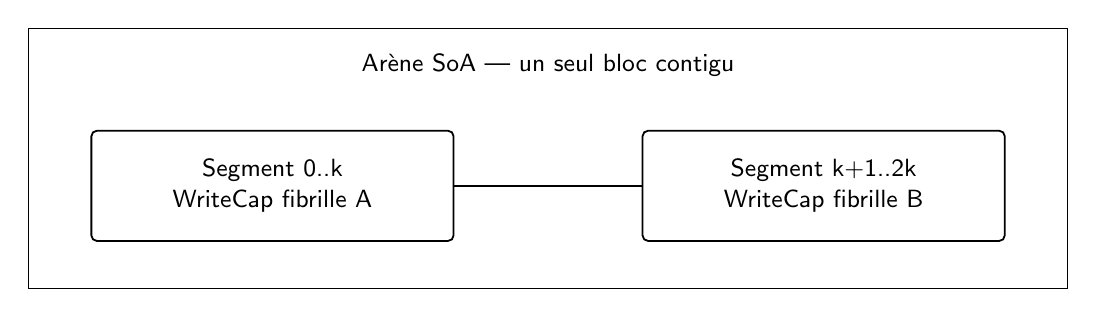
\begin{tikzpicture}[
  font=\sffamily\small,
  frame/.style={draw, line width=.5pt},
  box/.style={draw, rounded corners=2pt, align=center, line width=.65pt, minimum height=14mm, minimum width=46mm}
]
\draw[frame] (0,0) rectangle (132mm,33mm);
\node[anchor=north] at (66mm,31mm) {Arène SoA --- un seul bloc contigu};
\node[box] (a) at (31mm,13mm) {Segment 0..k\\WriteCap fibrille A};
\node[box] (b) at (101mm,13mm) {Segment k+1..2k\\WriteCap fibrille B};
\draw[line width=.65pt] (a) -- (b);
\end{tikzpicture}
\end{document}
